\documentclass[sigconf]{acmart}
\usepackage[utf8]{inputenc}
\usepackage{graphicx}
\usepackage{booktabs}

\setcopyright{rightsretained}

\acmConference[GECCO '17]{the Genetic and Evolutionary Computation Conference 2017}{July 15--19, 2017}{Berlin, Germany}
\acmYear{2017}
\copyrightyear{2017}


\begin{document}

\title[The EMeRGE modular robot]{The EMeRGE modular robot, an open platform for quick testing of evolved robot morphologies}

\author[R. Moreno]{Rodrigo Moreno}
\affiliation{%
  \institution{Universidad Nacional de Colombia}
  %\streetaddress{Cra 45}
  \city{Bogota} 
  \country{Colombia}} 
  %\postcode{111321}
\email{rmorenoga@unal.edu.co}

\author[C. Liu]{Ceyue Liu}
\affiliation{%
  \institution{China University of Mining \& Technology}
  %\streetaddress{Cra 45}
  \city{Beijing} 
  \country{China} 
  %\postcode{111321}
  }
\email{liuceyue@gmail.com}

\author[A. Faina]{Andres Faina}
\affiliation{%
  \institution{IT University of Copenhagen}
  %\streetaddress{Cra 45}
  \city{Copenhagen} 
  \country{Denmark}} 
  %\postcode{111321}
\email{anfv@itu.dk}

\author[H. Hernandez]{Henry Hernandez}
\affiliation{%
  \institution{Universidad Nacional de Colombia}
  %\streetaddress{Cra 45}
  \city{Bogota} 
  \country{Colombia}} 
  %\postcode{111321}
\email{heahernandezma@unal.edu.co}

\author[J. Gomez]{Jonatan Gomez}
\affiliation{%
  \institution{Universidad Nacional de Colombia}
  %\streetaddress{Cra 45}
  \city{Bogota} 
  \country{Colombia}} 
  %\postcode{111321}
\email{jgomezpe@unal.edu.co}

\begin{abstract}
This work presents the hardware design and implementation of the EMeRGE open modular robot platform. EMeRGE (Easy Modular Embodied Robot Generation) modules are designed to be cheap and easy to build and their hardware is open for anyone to use and modify. Four magnetic connectors enable the quick assembly of different complex robot morphologies like the ones generated by evolutionary robotics experiments. Non-human agents, like robotic manipulators, can also take advantage of the magnetic connectors to assemble and disassemble morphologies. 
%An example of how a morphology obtained using evolutionary algorithms is built using EMeRGE modules in reality is shown. 
\end{abstract}

%
% Remember to generate the code using the tool at
% http://dl.acm.org/ccs.cfm
% Please copy and paste the code instead of the example below. 
%
\begin{CCSXML}
<ccs2012>
<concept>
<concept_id>10010520.10010553.10010554.10010556</concept_id>
<concept_desc>Computer systems organization~Robotic control</concept_desc>
<concept_significance>500</concept_significance>
</concept>
<concept>
<concept_id>10010520.10010553.10010554.10010555</concept_id>
<concept_desc>Computer systems organization~Robotic components</concept_desc>
<concept_significance>300</concept_significance>
</concept>
<concept>
<concept_id>10010520.10010553.10010554.10010556.10011814</concept_id>
<concept_desc>Computer systems organization~Evolutionary robotics</concept_desc>
<concept_significance>300</concept_significance>
</concept>
<concept>
<concept_id>10010520.10010553.10010562</concept_id>
<concept_desc>Computer systems organization~Embedded systems</concept_desc>
<concept_significance>100</concept_significance>
</concept>
</ccs2012>
\end{CCSXML}

\ccsdesc[500]{Computer systems organization~Robotic control}
\ccsdesc[300]{Computer systems organization~Robotic components}
\ccsdesc[300]{Computer systems organization~Evolutionary robotics}
\ccsdesc[100]{Computer systems organization~Embedded systems}

\copyrightyear{2017} 
\acmYear{2017} 
\setcopyright{rightsretained} 
\acmConference{GECCO '17 Companion}{July 15-19, 2017}{Berlin,
Germany}\acmDOI{http://dx.doi.org/10.1145/3067695.3075616}
\acmISBN{978-1-4503-4939-0/17/07}

\keywords{Modular Robots, Morphology, Quick assembly, Magnetic connectors, Open hardware, Transferability}


\maketitle

\section{Introduction}
%Evolutionary robotics experiments are often done first in simulation and then tested in real robots. In contrast to transferring only controllers into predefined real robots, evolving and testing morphologies in reality involves a lot of effort and resources. Specially when each robot morphology to be tested can be very different from others. The introduction of rapid prototyping technologies such as 3d printing has helped reduce the resources associated with building and testing different robot morphologies in reality but it still can take a lot of time to print every part of a robot and assemble sensors and actuators into it. Evolutionary robotics experiments can take advantage of modular robot systems to test individuals in real life. Building robot morphologies using robotic modules in simulation has the advantage of being able to use the same type of modules in reality thus reducing the cost associated. Furthermore, by using basic blocks in simulation and in reality the difference in performance, or reality gap, could be reduced. In this work we study the differences between simulated robots evolved using modules as a basic element and their real implementation. For this purpose a new modular robot platform called EMeRGE (Easy Modular embodied Robot Generation) is designed and built. The EMeRGE module is designed to be easy to be assembled to other robots so that different morphologies can be tested in a quick way in reality. Modules are cheap and easy to build and their hardware and software is open for anyone to use and modify. An overview of the mechanical and electronic design is presented. By using basic blocks in simulation and in reality the difference in performance, or reality gap, could be reduced. 

When automatically designing the morphology and control of robots using evolutionary algorithms, solutions are usually tested in simulation but few are transferred to real robots. In contrast to transferring only controllers, evolving and testing morphologies in reality involves a lot of effort and resources. The introduction of rapid prototyping technologies such as 3d printing has helped reduce the costs associated with building and testing different robot morphologies in reality but it can still take a lot of time to print every part of a robot and assemble sensors and actuators into it \cite{Auerbach2014,Lipson2000}. Evolutionary robotics experiments can take advantage of modular robot systems to quickly test individuals in real life. The advantage is that simulated morphologies can be very quickly assembled using real modules, that can be reused, thus increasing the rate at which experiments can be made. In \cite{Faina2015} an evolutionary system is developed in which the goal is to evolve robots that can be assembled using modules. However, in this and other existing platforms building the modules themselves can still be a complex and expensive process and several are usually needed to build robots that can move to perform different tasks. Automatic connectors that come embedded in some prototypes are also difficult to build and increase the weight and energy consumption of the module. Even in the case of using manual connectors like in \cite{Faina2015} moving parts and screws increase the time to complete an assembly. A new modular robot platform, the EMeRGE (Easy Modular embodied Robot Generation) module is described in this work. EMeRGE modules are designed to be easily built using relatively cheap, commercially available components and their hardware design files are open for anyone to use and modify (see footnotes 1 and 2). Modules are easy to assemble to other modules, using magnetic connectors, so that different morphologies can be tested quickly in reality. Magnetic connectors are present in four faces of the module and infrared sensors which allow the EMeRGE platform to build more complex morphologies with more capabilities than similar open modular robot platforms \cite{Krupke2015}. The magnetic connector can also enable non-human agents, like robotic manipulators, to assemble and disassemble morphologies. The idea of using a robotic arm is also explored in \cite{Brodbeck2015} but with the use of glue to attach different modules making the disassembly process more difficult in turn. 
%Evolutionary systems trying to bridge simulation and reality like \cite{Koos2013} could potentially take advantage of the quick assembly feature to do more tests on real robots.
% * <frve@itu.dk> 2017-02-15T15:19:33.387Z:
% 
% > it still can take a lot
% *it can still take a lot
% 
% ^.

%Approaches using real robots to reduce the reality gap problem can benefit from this. Koos \cite{Koos2013}, for example, proposes creating a transferability function by testing in a real robot from time to time and interpolating the gap for individuals not tested in reality. However even when not testing every time, implementing morphology evolution in systems like this would take too much time when normal robots or even 3d printed robots are used. An attempt at automating the assembly process using glue is done in \cite{Brodbeck2015} but morphologies still take a lot of time to disassemble.
  
  %Automatic connector are more difficult to build and have more weight have more complex part. Even some manual connectors take time to assemble because they use moving  parts or screws.  
%Evolutionary robotics authors like Jakobi , Glette and Koos have identified possible causes and proposed methods to reduce it. Proposed methods can be classified in three categories: evolving directly in reality, creating more accurate simulators, and mixing real robot evaluations in the simulation loop. Some robot in the loop approaches have interesting results, 

%Jakobi \cite{Jakobi1995} indicates that simulations should include noise in the sensors readings and actuators so that evolved controllers for robots can cope with the differences. Small obstacles are used in simulation in Glette \cite{Glette2014}, in an analogy to Jakobi's noise, to test if they can lead to more robust controllers in an unconventional quadruped robot.  In this work we aim to study the differences between simulated robots evolved using modules as a basic element and their real implementation in order to see how the reality gap affect this kind of approach.

\section{The EMeRGE Modular Robot Platform}

The hardware of the EMeRGE module is designed for evolutionary and locomotion learning experiments. It allows for the quick assembly of different morphologies that can contain basic sensors. Different mechanical variations can be designed into the system so heterogeneous sets of modules can be used\footnote{The mechanical design can be found here: goo.gl/08LC79}. The module fits inside a 81x61x62mm parallelogram, and the module itself resembles a small cube with a central hinge. The central hinge is comprised of a Dynamixel AX-12A servo motor with a pair of brackets screwed to the motor axle and to its bottom. Also screwed to the brackets are two layers that act as faces for the cube, the first layer from the outside is a 3D printed plastic part that houses neodymium magnets and the second layer is a PCB in charge of routing communications and power to the other faces and the motor. The mating magnetic faces maintain mechanical and electrical connection. Only four faces of the cube possess connector faces being one of them male, the other two are purposefully left empty to let the central hinge move. Two joined faces can sustain up to 1.3 N.m of torque before complete disconnection. The motor has a maximum torque of 2.5 N.m.  
% * <frve@itu.dk> 2017-02-15T15:25:22.235Z:
% 
% > The hardware of the EMeRGE module is designed to be suitable for evolutionary and locomotion learning experiments, for this reason the design allows, as mentioned, for quick assembly of different morphologies and for the use of basic sensors.
% 
% Rephrase to two sentences? (It just didn't read very well...):
% The hardware of the EMeRGE module is deisigned for evolutionary and locomotive learning experiments. It allows for the quick assembly of different morphologies aided by the use of basic sensors. 
% 
% ^.

\begin{figure}
 \centering
 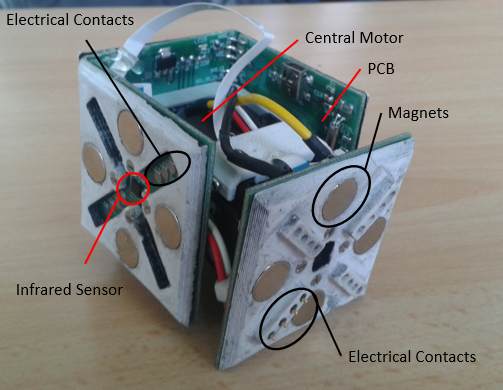
\includegraphics[width=0.8\columnwidth]{ModuleInd.png}
 \caption{\label{fig:module} The EMeRGE robotic module}
 \end{figure}

There are currently two implementations of the electronics \footnote{The electronics designs can be found here: goo.gl/EJNggy}, one that enables the control of the robots with as less components as possible and another that lets the robot do on board processing and sense the environment. The first routes signals directly from the Dynamixel AX-12A motor to the connector faces. The Dynamixel motor uses a multidrop half duplex serial communication scheme that can be daisy chained. Only three signals are needed: power, ground and data. Three of the PCBs are soldered to each other (see figure \ref{fig:module}) to provide mechanical stiffness and communication among them, the remaining PCB and the motor are connected by wires. Modules are powered by an external source which is routed to all modules through the connector faces. Modules must be connected to an external computer through a half duplex serial converter in order to be controlled.
% * <frve@itu.dk> 2017-02-15T15:44:48.377Z:
% 
% > Dynamixel protocol.
% Maybe add a reference to what this entails
% 
% ^.
% * <frve@itu.dk> 2017-02-15T15:42:52.962Z:
% 
% > with as less components as possible
% *with the least possible components
% 
% ^.
The second implementation of the electronics introduces an on board microprocessor, an 32 bit ARM\textregistered Cortex\textregistered-M PSoC\textregistered chip from Cypress. The microprocessor is capable of reading sensors, control the motor, and communicate with other modules. The chip can be programmed with different digital or analogue modules thus saving space in the PCB layout, i.e. a CAN controller can be programmed into the chip. A VCNL4010 infrared proximity sensor is also included at the center of each connector face (see figure \ref{fig:module}) and a CAN bus for communicating with other modules is implemented, although different communication protocols can be used. 



% This paper describes the design and implementation of the EMeRGE (Easy Modular embodied Robot Generation) modular robot and its use in quickly and easily deploying robots with different morphologies obtained by auto generating processes like evolution, identifying and closing the reality gap in evolutionary and learning experiments. By building robots from basic, simple parts, like modules, performance gaps can be reduced when transferring simulated controllers to real robots made from the same basic parts.   The robotic prototype is designed to be easy to be assembled to other modules so that different morphologies can be tested in a quick way in reality. An overview of the mechanical and electronic design is presented. The EMeRGE modules are cheap and easy to build and their hardware and software is open for anyone to use and modify, as tested by various research groups around the world. An experiment showing how the modules can be used to test evolved simulated morphologies in reality and a comparison between simulation and hardware experiments are discussed. Results show that both experiments sets are close/far away in their performance. In our case we want to test how the reality gap affects the evolved modular robot morphologies and controllers when transferred to real robots.
% Modular robot systems provide versatile solutions to many kinds of problems thanks to their reconfiguration ability. These systems have the main features of being scalable, robust and re-configurable.
% Simulation has been steadily growing as the tool of choice when performing evolution and learning experiments in robotics. However, simulated experiments have their limits, one of the most prominent being the reality gap problem. The reality gap is defined as the difference between the results obtained in simulation and the behavior observed in reality. This differences stem mainly form the heavy abstractions that have to be used when simulating robots like friction modeling and motor behavior.

% Modular robots are a subclass of multi robot systems that are built from basic units called modules, with or without autonomy and that can connect to each other in different ways an perform different tasks. Modular robots are often applied in evolutionary experiments due to the complexity of the robots that can be obtained by using basic parts. Modular robots experiments are often done in simulation due to limitations on the number of modules and the fabrication and building expenses of real modules.  Different modules include different ways in which to be connected to other modules, some of them enable the automatic connection and disconnection from each other, thus enabling self-reconfiguration, and others being completely manual or requiring an external agent to complete the assembly process.  Using a manual assembly strategy that lets modules be quickly assembled to each other opens the possibility of rapidly recreating simulated robots used for example in evolutionary experiments or learning experiments. The recreated robots can then be tested in real experiments and contrasted with their simulated counterparts. This can help identify key differences that increase the gap between simulation and reality.

%  There are different types of modular robots depending on how structures are organized when assembled. Chain type robot modules form chains when connected and can be arranged in rather arbitrary configurations, some chain type prototypes include PolyBot and CONRO, as well as the Y1 modules. Lattice type modules, as the name implies, connect to each other forming lattice or crystalline type structures, examples of this kind of modular robots include M-TRAN, ATRON and Molecube. Chain type modular robots have advantages over lattice type robots when generating locomotion movements. Most of these modular robot prototypes are controlled from an external computer. Design details are proprietary. Most modules are not easily built, and the ones that are, are not robust enough or offer a limited number of achievable assembly configurations, our solution is in the way between trying to make robust modules and keeping them as simple and easy to build as possible. Modules are also often not easy to repair

% Experiments involving evolution and modular robots focus mainly on evolving controllers for specific morphologies, specific ways to assemble a set of modules, to travel through flat environments. Others evolve the morphology itself for the same purpose. More recent works evolve control and morphology at the same time in order to achieve embodied beings (is this true?). Modular robots prototypes include M-TRAN, ATRON, REPLICATOR, and others and studies are mainly done in simulation.

\begin{figure}
 \centering
 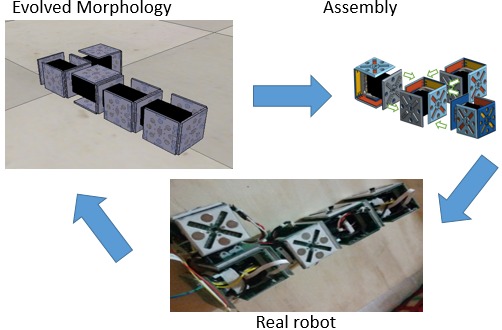
\includegraphics[width=0.8\columnwidth]{Assembly.png}
 \caption{\label{fig:assemb} Building of simulated morphology in roughly 25s.}
 \end{figure}


\section{From simulation to reality}%Insights gained


The EMeRGE module can be integrated into robot morphology evolution systems like in \cite{Veenstra2017}, in which modular morphologies are generated in simulation using different approaches. Figure \ref{fig:assemb} shows and example of how morphologies generated in simulation can be implemented as real robots in seconds. By taking advantage of the fast connection feature and other physical properties of the module, a robotic manipulator can be used to automate not only the assembly but also the disassembly process of morphologies obtained in evolutionary systems. This is an insight that we are currently exploring which can be advantageous for systems trying to bridge simulation and reality like \cite{Koos2013}. More EMeRGE morphologies can be seen here: http://vimeo.com/rodrm/emerge-modular-robot


%The EMeRGE module is simulated using the V-REP robot simulator. The simulated robot can be integrated into different robot morphology evolution systems like in \cite{Veenstra2017} in which modular robot morphologies are generated in simulation using a constructive approach with the Edhmor (Evolutionary designer of heterogeneous modular robots) system and L-systems. Figure \ref{fig:assemb} shows and example of how one of the generated morphologies in \cite{Veenstra2017} can be implemented as a real robot in a matter of seconds. The robots obtained can be tested against the same fitness measure as in the simulation and results compared. 



%Example showing how simulated morphologies can be obtained from the simulated systems and tested in reality (can use picture from liu videos) remember to upload video an reference it
%EMeRGE modules can be used to study the how the To study how the reality gap affects the performance of an evolved robot morphology based on the EMeRGE module first robots are evolved in simulation. Individual robots are evolved using the evolutionary algorithm described in \cite{Faina2013}. This system is built to evolve morphology and control of modular robots with different number of connecting faces and mechanical structures, in which solutions are highly deceptive. The task given to the robot is to move as far as possible from the starting position in any direction in a given amount of time so the fitness is represented as the distance moved. Due to restrictions on the number of robots generated morphologies can only have a maximum of 5 modules. The best performing individuals are built using hardware modules and the control parameters are transferred. Finally, the real robots are tested against the same fitness measure as in simulation and the results are compared. Results are expected to help identify the reality gap present in evolutionary robotics approaches that use modular robots as a basic building block in order to use a reality gap reduction method in the near future.

  


% \begin{figure}
% \centering
% \includegraphics[width=0.5\textwidth]{ThirdElec.png}
% \caption{\label{fig:ThirdE} Electronics diagram for the robotic module}
% \end{figure}

% \begin{figure}
% \centering
% \includegraphics[width=0.5\textwidth]{ThirdPCB.png}
% \caption{\label{fig:ThirdP} Electronics circuit board built}
% \end{figure}








% \subsection{1st Prototype}
%  The first prototype was built during the Master Thesis work, a detailed description can be found on: "Diseño y Simulación de un Algoritmo para el Control de un Robot Modular Tipo Cadena" published at Universidad Nacional de Colombia (Change for cite)

%  Main Features: The robot modules were built using bended aluminum sheets for the chassis, a central servo motor, an Arduino pro mini as a central controller, an Xbee radio for communication, and an accelerometer sensor 

%  \begin{figure}
% \centering
%  \includegraphics[width=0.5\textwidth]{First.png}
% \caption{\label{fig:first} First prototype}
%  \end{figure}

%  Eachmodule had to be connected by wires to an external power supply independently from each other and, even though the radios enabled the modules for wireless communication, the modules only talked with their nearest neighbors. Each module had only two connector faces, each face comprised 4 magnets and can connect in 4 different orientations to other faces, since the magnets have a north and a south pole faces were divided in male and female restricting the configuration to chains of motors in the same orientation. Worm or snake like structures, like the one in the picture were built and moved by means of a bio-inspired control algorithm in which there is no central controller but rather each module synchronizes with its neighbors.
% % * <frve@itu.dk> 2016-12-07T17:17:47.421Z:
% %
% % > bio-inspired control algorithm
% %
% % Do you know of any other algorithms that are similar? And do you have an example from Biology? I know that people think that some worms move through local interactions between segments but higher organisms tend to have a centralized control structure where motor neurons from the brain or spinal cord move towards muscle tissue. 
% %
% % ^.

%  \subsection{2nd Prototype}
%  A second module prototype was developed during the ITU stay in 2014-2015. The whole prototype was redesigned from the motor to the external connector, to the communication scheme. The second prototype was based in the Dynamixel AX-12A servo motor by ROBOTIS. The AX-12A servo motor has a higher torque than the previous servo motor used, and can be controlled using a multidrop serial communication interface that can be daisy chained

%  Since the motor serial interface supports a three signal scheme the connectors for the modules were adapted with electrical contacts in the form of screws maintaining the male-female order.

%  \begin{figure}
%  \centering
%  \includegraphics[width=0.5\textwidth]{SecMaleFemale.png}
% \caption{\label{fig:SecC} Male and Females connector faces for the second prototype, faces are laser cut from a POM sheet and are based on the Dynamixel network signals}
% \end{figure}

%  Thecolored points on figure \ref{fig:SecC} indicate the signals running through the corresponding screws. Power is transmitted through the connector screws so all modules can be powered from a single point in the structure. Two more connector faces were added to the sides of the motor enabling the assembly of more and different structures.

% \begin{figure}
% \centering
%  \includegraphics[width=0.5\textwidth]{SecAssem.png}
% \caption{\label{fig:SecA} Complete assembly of second prototype module design}
%  \end{figure}

%  Cantileversprings were added to the male connectors to ensure electrical contact under different torque conditions.
%  Magnetsare still used to join the faces but this time 8 magnets are used instead of just 4, magnets are fixed inside the connector face by friction forces and the magnetic poles are alternated to ensure that the connector aligns its sides and electrical contacts with its companion. Each connector face was laser cut from a 3mm POM plastic sheet

%  The connector assembly (one connector face joined to another) can maintain its connection up to a torque of 1.7 N.m. Different configurations were assembled using 8 modules built with this design. Connections inside the module are completely wire based which resulted in disconnection of some parts after some movement tests.

% \begin{figure}
%  \centering
%  \includegraphics[width=0.5\textwidth]{SecStruct.png}
% \caption{\label{fig:SecS} Real structure built using the second prototype modules}
% \end{figure}

% \subsection{3rd Prototype}

%  Thethird prototype design is based on the second one. Connector faces are redesigned to be 3D printed and electrical contacts are moved from the sides of the face to the center, the male-female order is still maintained.

%  Electricalcontacts are maintained by means of a spring pin connector which is soldered to a PCB behind the 3D printed face.

%  The PCB behind the 3D printed faces is in charge of routing power and communications to the motor and, in the most simple version, it can work with the Dynamixel serial multidrop version as in  the second prototype. A more elaborated electronics design is being developed right now, the electronics are based on a single microcontroller per chip that can read proximity sensors, control the motors, and communicate with other modules via CAN bus. 

%  The design uses VCNL4010 sensors for proximity measurement, and a Cypress PSOC chip as a central controller. The PSOC chip works like a programmable hardware device which lets different types of modules be embedded in one chip, i.e the CAN controller, the half duplex serial converter and the I2C multiplexer are implemented inside the central chip. The elaborated controller design can let the motor be controlled directly with the Dynamixel serial network, or use the central chip and the CAN bus for communications. As in the second prototype, power is routed through the connector faces so the whole robotic structure can be powered from a single point. 



%  Only 4 magnets are used in the third prototype connector face design but 12mm magnets are used instead of the 8mm old ones, getting a max disconnection torque of 1.3 N.m similar to the double magnet case.

% \subsection{Main Advantages of the Robotic Module}
% The main advantages of the module include:

% \begin{itemize}
% \item The module is tailored towards easy evolution of configurations and locomotion learning experiments
% \item The module design can be easily modified, and its open for anyone to improve.
% \item It provides more connector faces and communication reliability than other 3d Printed Modules.
% \item Can help reduce the reality gap since it is simple to simulate and easy to assemble.
% \item It is relatively cheap and easy to build, and its parts are also cheap and easy to build.
% \item Extra different modules can be designed and attached to the robotic structures.
% \item Can be assembled and disassembled automatically (Pending).
% \item Modules can process information and actuate by themselves or they can be controlled by an external computer.
% \item New modules can be added at any time.



% \end{itemize}


% \section{Discussion and Future Work}
% What we expect to have working in the future and the applications we want the robot to tackle

\begin{acks}

This work was supported in part by \grantsponsor{GS501100002945}{Direcci\'on de Investigaci\'on, Universidad Nacional de Colombia}{http://dx.doi.org/10.13039/501100002945} under Grant No.:~\grantnum{GS501100002945}{23418}. The authors thank Frank Veenstra for his helpful discussion.

%This project was supported in part by grant 23418 of the program "Programa nacional de proyectos para el fortalecimiento de la investigaci\' on, la creaci\' on y la innovaci\' on en posgrados en la Universidad Nacional de Colombia 2013" of Universidad Nacional de Colombia.
\end{acks}


\bibliographystyle{ACM-Reference-Format}
\bibliography{HardwarePaper2017.bib}

\end{document}
